\documentclass[utf8]{../IncArticle}
\graphicspath{{../}}
%\usepackage{color}
%\usepackage{todonotes}
% \usepackage{lmodern}
\usepackage{xcolor}

\colorlet{pcolor}{blue}
\colorlet{fcolor}{red}
\newcommand{\e}[2][fcolor]{\textcolor{pcolor}{[}\textcolor{#1}{#2}\textcolor{pcolor}{]}}





% *** PDF, URL AND HYPERLINK PACKAGES ***
%
\usepackage{url}

\title{Интерактивная методика извлечения семантической разметки
  текстовых документов, основанная на полисистеме онтологий
  \e{Первоначальный заголовок: Методика ПРИОБРЕТЕНИЯ знаний из
    текстовых документов, основанная на анализе ответов пользователя и
    полисистеме онтологий} }

% \AddAuthor{Черкашин}{Е}{вгений}{А}{лександрович}{Институт динамики систем и теории управления СО РАН, Иркутск, ул. Лермонтова 134, 664033}
% \AddAuthor{Черкашин}{А}{лександр}{К}{онстантинович}{Институт географии им. В.Б. Сочавы СО РАН, Иркутск, ул. Улан-Баторская 1, 664033}
% \AddAuthor{Бычков}{И}{горь}{В}{ячеславович}{Институт динамики систем и теории управления СО РАН, Иркутск, ул. Лермонтова 134, 664033}
% \AddAuthor{Паскал}{К}{ристина}{К}{онстантиновна}{Национальный исследовательский Иркутский государственный технический университет, Иркутск, ул. Лермонтова 83, 664074}
% \AddAuthor{Белых}{П}{олина}{В}{асильевна}{Институт динамики систем и теории управления СО РАН, Иркутск, ул. Лермонтова 134, 664033}

\AddAuthor{Черкашин}{Е}{вгений}{А}{лександрович}{}
\AddAuthor{Черкашин}{А}{лександр}{К}{онстантинович}{}
\AddAuthor{Бычков}{И}{горь}{В}{ячеславович}{}
\AddAuthor{Паскал}{К}{ристина}{К}{онстантиновна}{}
\AddAuthor{Белых}{П}{олина}{В}{асильевна}{}

\setcounter{page}{1}
\date{}
\begin{document}

\begin{abstract}
%\boldmath

  В докладе представляется идея подхода к представлению и индукции
  логического слоя представления содержимого, например, сайтов,
  юридических документов и т.п. Этот слой порождается на основе
  анализа результатов редактирования содержимого (контента) --- как
  текстовой составляющей, так и его существующей логической структуры.
  Варианты интерпретации того или иного изменения содержимого
  (исправление ошибки/значения или формирование нового высказывания)
  уточняются при помощи диалога с пользователем.  На принятие решения
  также влияют результаты анализа поведения пользователя, например,
  выделяются повторяющиеся переходы между редактируемыми документами
  определенных классов.

  Теоретической основой методики является представление предметной
  области в виде полисистемы онтологий, т.е. многослойной структуры
  понятий и отношений, которые отображаются между слоями через
  интерпретацию.  Полисистема онтологий, представленных в виде
  семантических сетей, позволяет организовать диалог с пользователем,
  упорядочивать и классифицировать факты о предметной области, а также
  получать новые интерпретации формируемых концептов.

  В качестве тестовой среды для разрабатываемых технологий выбрана
  автоматизация деятельности нотариальной конторы и документооборот
  административных, хозяйственных и научных подразделений бюджетного
  учреждения.  Документы, используемые в этих видах деятельности,
  обладают одним важным свойством --- содержащаяся в них информация
  представляется как в структурируемом, так и в неструктурируемом
  виде.

\end{abstract}

\begin{abstract}[english]
  \e[blue]{Here we have English abstract}
\end{abstract}


\introduction{}

В 2001 году Т.~Бернерс-Ли предложил план развития интернет"=технологий
(семантический веб), который направлен на реализацию сетевых сервисов
со значительным уровнем интеграции логического слоя представляемой
информации.  Информация размечается семантически, а программные агенты,
используя эту информацию, производят ее обработку с целью решения
конкретных практических задач пользователя.

Одной из основных проблем семантического веба является тот факт, что
большинство пользователей решают свои практические задачи и не
заинтересованы повышении своей квалификации до уровня позволяющего
использовать эти технологии в полной мере.  В такой ситуации
технологические аспекты семантического веба должны быть полностью
скрыты, а программное обеспечение должно "варить кашу из
топора".  Необходимо разрабатывать программное обеспечения управления
содержимым сайтов и юридических документов как технологий приобретения
знаний, где пользователю предоставляется роль источника дополнительной
информации для интегрированного в систему механизма поддержки принятия
решений.

В настоящее время распространены два подхода к разметке текста
документа: а) совместное использование формата HTML и RDFa; б)
\e{специальное} распознавание интерпретация комбинаций атрибутов HTML
без использования каких-либо расширений HTML.  Первый подход является
результатом планомерного развития технологий СВ.  Сформирован ряд
классов языков представления семантической
разметки, различающихся по выразительности, сложности синтаксиса,
сложности алгоритмов обработки, разрешимости соответствующих
\e{логических формализмов} логик описаний (description logics).
Второй подход направлен на создание программной среды обработки
семантических данных, обеспеченных вычислительно несложными
алгоритмами и гарантированной разрешимостью соответствующих логических
\e{задач}.  Технология микроформатов \cite{b2:2} --- наиболее
известный представитель данного направления.  Микроформатные данные
обрабатываются на стороне клиента (в веб-браузере) при помощи
встроенных (plug-in) модулей.  Общим элементом обоих подходов ---
использование HTML в качестве формата представления текстовой
информации, а также сетевого формализма представления данных знаний
\e[cyan]{развивать мысль дальше? тройки, графы ...}.

Идею предлагаемого подхода к автоматизации извлечения семантической
разметки удобно излагать на примере юридических документов, которые в
большинстве случаев содержат сведения об отношениях между физическими
и юридическими лицами, а также другими элементами.  Эти сведения в
исходной или преобразованной форме используются в других документах.
Поэтому имеет смысл для каждого документа извлекать и хранить
достаточно детально представленное логическое описание таких сведений,
которое преобразуется в текстовый документ при помощи шаблонов.
Вариант преобразования определяется отображаемым документом,
т.е. документ задает контекст представления логического слоя.

К настоящему времени технологии Семантического Веба (СВ) предоставляют
формальные механизмы представления указанных отношений при помощи
стандартных форматов и структур данных, а также несколько механизмов
их логической обработки.  Логический слой представления информации в СВ
представляет собой граф, состоящий из концептов (понятий) и отношений
между ними.  В частности в юридическом документе физические и
юридические лица находятся с этим документом в отношении
``часть--целое'', а также в их более точных и содержательных вариантах.

В настоящее время большинство вариантов использования онтологических
моделей предметных областей сводятся к решению задачи уточнения
диапазона релевантных документов в процессе поиска.  Автоматизация
извлечения онтологий из текстовых документов базируется на
сканировании хранилищ документов: содержимого текста документов и их
метаданных, анализ результатов сканирования.  Наблюдение за поведением
людей в процессе подготовки различных документов приводит к
заключению, что содержательные части документов, которые и
представляются в логическом слое, как правило, находятся в тех местах
текста, где чаще всего пользователи производят изменения.  Поэтому,
информационная система, автоматизирующая процессы подготовки
документов, должна отслеживать изменения, вводимые пользователем, во
времени и в пространстве версий.  Версии порождаются копированием
документа или использование его в виде шаблона нового
документа.  Подвергаться анализу должна вся совокупность
изменений.  Предлагаемый подход позволяет сузить объем обрабатываемой
информации за счет фокусировки алгоритмов анализа данных вблизи
изменений.  Границы изменений задаются, например, свойствами формата
представления текста документа (гипертекстовой разметкой) или
существующей логической структурой одной из его \e{документа} версий.

Элементы логического слоя (концепты, объекты и отношения между ними)
формируются в результате применения алгоритмов анализа данных и
интервьюирования пользователя.  Среда, контекст, \e{приобретения знаний}
включает в себя:
\begin{itemize}
\item полисистему онтологий, совокупно описывающую предметные области,
  имеющие отношение к представлению документа как структуры данных,
  так и его содержательного смысла;
\item история изменения документа и его логического слоя;
\item список последних изменений в текущей транзакции (новой версии);
\item история действий пользователя в системе (пользователь, например,
  выполняет типичный набор действий по подготовке стандартного пакета документов);
\item ответы пользователя на утоняющие вопросы системы, цель которых
  --- определить \e{истинные намерения пользователя} смысл сделанных исправлений.
\end{itemize}

В результате анализа этих данных формируются новый набор троек вида
\texttt{<subject, relation, object>}, \e{представляющих новые данные
нового документа/версии, представленные в логическом
слое}.  Накопленные логические слои документов необходимо периодически
также сканировать на выявление стойких функциональных зависимостей
между значениями объектов.  В результате этого анализа, предлагается
совершенствовать формат представления данных слоя, например применяя
реляционные таблицы в качестве хранилищ.  \e{Метод функциональных
зависимостей применяется наоборот (т.е. данные - анализ - структура)}.

Сеть взаимодействующих программных систем, в которых реализованы
перечисленные функции, обладает многими свойствами социальной сети.
Основными видами обработки информации в такой сети являются ввод,
хранение, фильтрация и передача, т.е. интеграция данных, а не их
агрегация с целью порождения комплексных отчетов.  Поэтому применения
специальных методологий проектирования программного обеспечения при
разработке таких систем (или подсистем приобретения знаний
описываемого вида), например, объектно"=ориентированных технологий, не
является значительным преимуществом.  Гораздо важнее обеспечить
возможность функционирования программ в доступной недорогой серверной
среде (хостинге) и создания каналов данных на основе современных
стандартных форматах данных и сетевых интерфейсов прикладного
программирования.  Обработку информации агрегированного типа в
социальных сетях выполняют, преимущественно, пользователи и, как
правило, подсознательно.

Интересным свойством такой социальной сети, реализующей, фактически,
распределенный документооборот, является требования к организации
обмена данными между пользователями в процессе подготовки документов
преимущественно в режиме off-line.  Современные информационные
технологии позволяют хранить данные логического слоя в разметке
электронных документов \ref{microformats,RDFa} и в виде QR-кодов,
сопровождающих печатные варианты документов.

В качестве платформы для тестирования разрабатываемых технологий
выбрана автоматизация деятельности российского нотариального
офиса.  Операции, выполняемые над документами и шаблонами представимы
как изменения содержания текста документа и его логического
слоя.  Примерами таких операций выступают копирование логического слоя
из одного документа в другой, смена ролей лиц в документа в процессе
его подготовки, накапливание базы данных клиентов и другой справочной
информации, \e{доступ к которой организуется при помощи быстрого
контекстного поиска}. \e[green]{Далее содержимое сайтов и документов будем
просто называть просто ``документ''}.

\section{Представление логического и презентационного слоя документа}

Стандартный формат представления знаний RDF описывает информационные
ресурсы при помощи троек вида \texttt{<subject, relation, object>} в
некотором контексте.  Множество всех троек задают некоторый граф (сеть)
объектов и концептов, а также отношений между ними, формируя систему
знаний предметной области.  Такое описание предметных областей удобно
разбивать на подграфы, организовывать их в иерархические комплексы
\cite{b4}, порождая иерархии контекстов.  В общем случае, контекст
влияет на способ или вариант интерпретации троек.  Например, фамилия и
данные паспорта в нотариальных документах могут располагаться в разных
частях текста, однако относятся к одному контексту --- личным данным
пользователя.  \e{Ну и что за странный пример??}

В предлагаемом подходе [-2-] шаблоны для отображения логического слоя
документа также хранятся в графе.  При помощи троек задаются
представления (views) и алгоритмы функциональных отображений,
например, контроллеров (controllers) в рамках шаблона проектирования
MVC (Model View Controller) \cite{b2:5}.  \e{На рис.~\ref{listex}}
представлен пример представления разметки текста (личная информация о
человеке) в формате FOAF (Friend of a Friend), а также часть его
шаблонов представления.

\begingroup%
\tt%
\begin{verbatim}
<rdf:RDF
 xmlns=”http://www.w3.org/1999/xhtml”
 xmlns:rdf="http://www.w3.org/1999/02/22-rdf-syntax-ns#"
 xmlns:foaf="http://xmlns.com/foaf/0.1/"
 xmlns:s="http://www.w3.org/2000/01/rdf-schema#"
 xmlns:view=”http://purl.org/aquarium/engine/MVC”
 xmlns:tal="http://xml.zope.org/namespaces/tal">
  <rdf:Description rdf:about="http://www.example.com/People/II/contact#me">
    <rdf:type rdf:resource="http://xmlns.com/foaf/0.1/Person"/>
    <s:seeAlso rdf:resource="http://www.exam..../People/II/contact"/>
    <foaf:homepage rdf:resource="http://www.example.com/People/II"/>
    <foaf:img rdf:resource="http://www.example.com/people/II.png"/>
    <foaf:mbox rdf:resource="mailto:ii@www.example.com"/>
    <foaf:name lang=”en”>Ivan Ivanov</foaf:name>
    <foaf:name lang=”ru”>Иван Иванов</foaf:name>
  </rdf:Description>
  <!— Представление данных физического лица в  HTML+RDFa. -->
  <rdf:Description rdf:about="http://xmlns.com/foaf/0.1/Person">
    <view:pt xml:lang=”ru”>
      <--! Тег view:pt задает формат представления -
           pt (Zope Page Template). -->
      <--! Значение переменной “subj” - это субъект тройки. -->
 <a href=”.” tal:attributes=”href rdf: subj s:seeAlso”
  tal:omit-tag=”not: rdf: subj s:seeAlso”>
       <span tal:replace=”rdf: subj foaf:name”/>
      </a><br/>
 Home page: <a href=”” tal:attributes=”href rdf: subj foaf:homepage”>
  <span tal:replace=”rdf: subj foaf:homepage”/>
      </a><br/>
 E-mail: <a href=”mailto:me@example.com”
           tal:attributes=”href string:mailto:${rdf: subj foaf:mbox}”>
 <span tal:replace=”rdf: subj foaf:mbox”/></a>
    </view:pt>
  </rdf:Description>
</rdf:RDF>
\end{verbatim}%$
\endgroup

В первой части приведенного примера задан экземпляр класса
\texttt{Person} (контактные данные конкретного человека --- Ивана
Иванова) как элемент графа онтологии.  Вторая часть примера ---
описание представления ресурсов класса \texttt{Person}.  В качестве
механизма \e{заполнения шаблонов} использована усовершенствованная
версия механизма Chameleon.  Механизм интерпретирует запросы
\texttt{rdf:} к графу семантики как строковые выражения, подставляемые
в шаблон HTML, или заменяемые его некоторые конструкции.  Шаблону
передается набор глобальных переменных, обозначающих субъект
(\texttt{subj}), который отображается, его контекст/контейнер
(\texttt{container}), собственно сам шаблон (\texttt{template}).  В
представленном примере \texttt{subj} указывает на экземпляр класса
\texttt{Person}, а \texttt{context} казывает на документ, в котором
упомянут данный экземпляр.  При помощи переменной \texttt{template} в
шаблоне доступны различные константы и дополнительные данные, которые
\e{помогают} процессу отрисовки текста.

Поддержка структур данных троек реализована как расширения синтаксиса
механизма TALES (Template Attribute Language Expression
Syntax). Определен новый вид выражений \texttt{rdf:}, вид которых
определен исходя из традиций стандарта RDF (стандартные
идентификаторы, пространства имен и т.п.) и синтаксиса логических
языков логик описания (логические связки, вид выражений).  Дополнение
Chameleon также коснулись механизма порождения результирующего
текста. Результаты выполнения выражений обрамляются разметкой
логического слоя при помощи структур RDFa, что позволяет, например,
передать на сторону клиента информацию о разметке и использовать при
формировании пользовательского интерфейса для редактирования элементов
логической разметки.

При реализации интерфейса пользователя необходим механизма определения
функциональных отношений алгоритмически.  Для этого в граф вводятся
методы, а также их реализации на разных языках.  В следуем примере при
помощи метода \texttt{nameUpcased} определяется функция представления
имени человека большими буквами.  Для метода заданы две реализации в
языках Python и JavaScript.

\begingroup
\tt
\begin{verbatim}
<rdf:RDF xmlns:html=”http://www.w3.org/1999/xhtml”
  xmlns:rdf=http://www.w3.../22-rdf-syntax-ns#
  xmlns:foaf="http://xmlns.com/foaf/0.1/"
  xmlns:s=http://www.w3..../rdf-schema#
  xmlns:view=”http://purl.org/aquarium/engine/MVC”
  xmlns:tal="http://xml.zope.org/namespaces/tal">
  <rdf:Description rdf:about="http://xmlns.com/foaf/0.1/Person">
    <view:method html:id=”nameUpcased”>
       <html:script type="text/python" xml:lang=”ru”>
  <--! Экземпляр передается в параметр “self” -->
   return self[“foaf:name”][0].upper()
       <html:script>
       <html:script type="text/javascript" xml:lang=”ru”>
  <--! Экземпляр задается переменной “this” -->
   return this.query(“foaf:name”)[0].toUpperCase()
       <html:script>
    </view:method>
  </rdf:Description>
</rdf:RDF>
\end{verbatim}
\endgroup

Ограничение прав доступа также реализуются по аналогии с
представленным в \cite{b2:6,b2:7}, используя данные, представленные
также в виде троек RDF.

Содержимое документа в общем случае представляется в виде дерева, где
большинство узлов являются и субъектами и объектами
одновременно. Исключения составляют корневой узел (он является только
субъектом) и листовые узлы (только объекты).  В иерархии документов
корневые узлы связаны \e{другими} отношениями, например, организацией
документов в тематические иерархии и кластеры.

Одним из основных моментов исследования --- это разработка методики
адаптации процесса извлечения разметки к процессу редактирования
документа.  Далее будем предполагать, что изменение, вносимое
пользователем, влияет на содержательный смысл текста документа
(изменяемой структуры), соответственно изменяя его логический слой.
Т.е. мы далее не рассматриваем простое исправление ошибки, которое
представляет собой изменение значения поля \texttt{object} и только
его в тройке, или исправление текста абзаца, в том числе в исходном
шаблоне.  Содержательное изменение в основном приводит к формированию
новой тройки между каким-либо субъектом в контексте документа и
изменяемым значением.  Анализ изменений в тексте документа направлен
на формирование таких новых данных и знаний, при этом система играет
активную роль, а пользователь является источником дополнительной
информации.

Обогащение семантической разметки в среде, содержащей логическую
структуру исходного документа, которая уже храниться в базе данных.  И
тогда перечень данных, используемых системой для принятия решения
включает\,:
\begin{enumerate}
\item исходную версию документа;
\item изменения текста документа, представленные в виде стандартного
  diff-формата \cite{b9};
\item ответы пользователя на вопросы, задаваемые системой; ответы
  уточняют смысл изменений (\e{что имел ввиду пользователь});
\item перечень действий пользователя, предшествовавших данному
  исправлению документа. \label{em:behav}
\end{enumerate}
Суть п.~\ref{em:behav}, например, проявляется при создании нового
документа из шаблона или его копии, что вообще говоря, приводит к
необходимости заполнения определенного перечня полей \texttt{object}
уже существующих троек.  Таким набором, например, выступает
стандартный набор полей для идентификации физического лица (ф.и.о.,
данные паспорта, адрес места жительства и т.п.) в нотариальной
доверенности.

Если же документ модифицирован частично, то данное изменение
интерпретируется как (\e{если это не простое исправление ошибки}) \e{a refinement of the logical structure of subject, extraction of a relation and an object; this corresponds to a new triple connecting the subject to the new object (changed value); the user must choose the \e[blue]{subject} of the new triple.}

Новый субъект должен быть выбран из списка (дерева) всех существующих
в контексте документа субъектов.  Далее для этого субъекта формируется
список всех возможных отношений, который формируется из всех возможных
отношений для этого субъекта и его класса, включая классы-предки.
Пользователю необходимо выбрать одно отношение для формируемой тройки.
\e{Надо где-то сказать про то, как сужать данный список.}  Если в
списке не содержится необходимого отношения, то его необходимо
определить.  \e{Что-то про определение...}  Новое отношение является
всегда \e{уточняющим} подклассом какого-либо существующего в списке
отношения.  Чтобы не \e{загрязнять} систему новыми сущностями\e{,
обозначающими отношения,} сформированными неопытными и невнимательными
пользователями, необходимо периодически проводить анализ этих
отношений инженерами знаний.  Их задача исключить дублирующие (эквивалентные),
противоречивые и семантически неточные отношения, и производить
реорганизацию (refactoring) онтологической модели.

Если объект какой-либо тройки удален, то и вся тройка должна быть
также удалена из логического представления документа.  Процесс
удаления должен контролироваться анализом минимальной структурной и
семантической непротиворечивости.  Например, при удалении из
доверенности физического лица, должны быть удалены и его паспортные
данные (\e{другое дело - имеет ли смысл удалять физ.лицо из
  доверенности.}). В результате анализа либо удаление разрешается,
либо запрещается, либо создает цепочку удалений троек, как в примере с
физическим лицом.  Для реализации этой функции каждый класс субъектов
необходимо сопроводить перечнем троек, которые необходимы для
формирования его содержательного базиса.

Добавление троек, в общем случае, приводит к добавлению новых
субъектов и отношений.  Примером такой ситуации выступает создание
трехстороннего договора из двустороннего добавлением нового физического
лица.  При этом также необходимо, в общем случае, заполнить
необходимые поля паспортных данных, а также установить отношения между
контекстом, субъектами документа и новым физическим лицом.

\section{Теоретическое обобщение процесса извлечения разметки}

Вышеописанный процесс является пошаговой реализацией процедуры
полисистемного анализа и синтеза \cite{father} (ППАС), которая
является общей процедурой системного анализа предметных областей.
Суть процедуры состоит в том, что предметная область и все ее объекты
и процессы расслаиваются по солям и представляются концептами и
отношениями (морфизмами) в многомерном пространстве слоев-координат.
В отличие от классического системного подхода, где принцип
взаимодействия элементов является фундаментальным, полисистемный
анализ предполагает выполнение гипотезы расслоения, т.е. он
предполагает, что объект исследования представим в виде
заимонепересекающихся слоев (подмножеств в частном случае),
подобластей. \e{Что там с концептами, отношениями, морфизмами интерпретациями??}  Таким образом, полисистема и является системой сама по
себе с более общей точки зрения, а ППАС --- это новый вид системного
анализа.

В общем виде приложение ППАС к задаче автоматизации построения
разметки документов состоит в построении многослойной декомпозиции
предметной области и данных документа. В качестве слоев выступают
различные аспекты представления документа\,: структурная
(мереологическая) организация документа, концептуальное моделирование
предметной области документа, наследование свойств документов,
моделирование отношений между физическими и юридическими лицами,
модели документов в \e{дионическом представлении} и т.п.

В соответствии с ППАС \cite{father} каждому концепту одного слоя
полисистемного расслоения должен соответствовать (через интерпретацию)
концепт во всех других слоях, а также отношения с другими концептами в
его слое.  В идеальном случае в каждом слое в результате выполнения
процедуры должна быть построена законченная теория.  Все теории
\e{отличается своими фундаментальными основаниями}, но также являются
схожими через интерпретацию (подстановку, замену) концептов.  Все это
позволяет нам индуцировать (порождать) новые аксиоматические теории
предметных областей по образу и подобию уже построенных.  Каждый
системный уровень (слой) знаний также многократно и последовательно расслаивается,
порождая полисистемное представление исследуемого объекта.  Таким
образом, все системные теории комбинируются в объединенную модель,
описывающую и предметную область и объект исследования.  \e{в нашем
  случае --- документ.}

В нашем случае ППАС направлена на порождение (формирование) троек и
контекстов (слоев).  Получаемые классы документов, физических и
юридических лиц и других объектов формируют множество концептов
теории соответствующего слоя.  Выделяя новый класс или отношение между
классами, необходимо \e{обязательно} установить связь с концептами и отношениями в
других слоях (интерпретацию).  Для удобства восприятия необходимо
также создавать для получаемых концептов определения на естественном
языке, соответствующее слою.

Each of new concept (a class) as we described in the previous section
is to be inherited from a parent class, thus, it can be interpreted in
other ontologies as either a concept that corresponds to the parent
class or to a new inherited class.  This case the user interview also
organized to obtain a description of the class and the relation.

Использование ППАС позволяет нам \e{справиться с} полнотой понятий и отношений
порождаемого слоя (\e{описания и его теории}) (\e{как это в диссертации Ковалева}
\ldots{} \cite{sergey}), а также непротиворечивости (при помощи
верификации онтологии).

\subsection{Ведение диалога с пользователем}

\e{... на базе полисистемы онтологий.}

Как было сказано выше, любая моделируемая предметная область \e{может
  быть} декомпозирована в полисистему понятий, объектов и отношений. С
общей точки зрения полисистема --- иерархическая структура,
составленная из непересекающихся слоев.  Каждый уровень включает
систему концептов, объектов и отношений между ними.  В уже
расслоенной полисистеме концепты одного уровня через
морфизм-интерпретацию отображены в концепты других уровней.  Все
концепты также через интерпретацию отображаются на концепты
абстрактного системного слоя.  Свойство отображения концептов между
слоями через интерпретацию \e{должно быть использовано} в качестве
основы реализации диалоговой подсистемы взаимодействия с
пользователем.  При этом при помощи рассуждения по аналогии,
представляемое в полисистеме онтологий как анализ структуры отношений
в слое и движение вдоль отношений и интерпретационных отображений
(между слоями).  \e[cyan]{Похоже на повторение при прямом прочтении
  текста статьи.}

Рассмотрим простой пример модели семейных отношений, изображенный на
рис.~\ref{OPSA} (на рисунке большинство очевидных отображений
интерпретации не отображены).  Полисистема, изображенная на рисунке,
включает четыре слоя, которые представляют собой различные модели
семьи Боба.  Слой 1 представляет семью как конкретный объект, в этом
слое содержатся только a-box-элементы \cite{abox}.  Слой 2 задает
основные роли (отношения) членов семьи. Слой 3 представляет \e{genders
  as two opposites}. Слой 4 отображает мереологическую концепцию,
т.е. суть отношения ``часть--целое''.

Попробуем построить на основе этой полисистемы онтологий список
вопросов, при помощи которых определяется, какую роль в семье Боба
играет Джул \e{(Юля)}.  Предположим, что уже известно, что Джул ---
женщина.  Чтобы поместить Джул в слой 1 необходимо задать вопрос
пользователю\,: ``Является ли Джул частью семьи Боба?''.  Вопрос
порождается в результате индуктивного вывода о том, что все отношения
в семье через интерпретацию отображаются на отношение ``являться
частью:'' слоя 4.  Это \e{наблюдение} моделируется контравариантным
функтором из слоя (категории) 2 в слой 4 (показано на рисунке
стрелкой от отношения ``бытьОтцом:'' к ``partOf:'', другие аналогичные
стрелки не изображены).  Теперь для того, чтобы подтвердить факт, что
Джул --- член семью Боба достаточно спросить\,: ``Правда ли, что Джул
являетьсяЧастью: Семьи Боба?''.  Обозначение экземпляра ``Семья''
можно сформировать по традиционному принципу обозначения семьи именем
отца семейства (ОС), т.е. именем ``Боб''.  Данный факт обозначен на
рисунке стрелкой от Боба в слое 1 к концепту ``ОС'' слоя 2.

Если пользователь ответил на данный вопрос утвердительно, т.е. Джул
является частью семьи Боба, то нам нужно далее уточнять роль Джул, так
как отношение ``partOf:'' не используется (\e{запрещено к
  использованию}) в слое 1.  Джул --- женщина, поэтому не может быть
ни отцом не сыном. Если бы это было так, то она должна быть мужчиной,
но мужчина и женщина --- формально противоположные концепты.  Если для
отношения ``бытьМатерью:'' в слое 1 задана кратность, то уже будет
известно, что в семье уже есть мать Алиса.  Поэтому остается один
вариант задать вопрос:''Джул [играет роль] дочери в семье Боба?''.  И
теперь, если ответ будет утвердительный, то создается новая тройка: \texttt{<Bob's-family hasDaughter: Jul>}.

Если, например, пол Джул неизвестен, то второй вопрос синтезируется
следующим образом: ``Какую роль играет Джул в семье Боба?''.  В
качестве вариантов ответа выдается список из двух отношений:
``hasDaughter:'' and ``hasSon:''.  \e[cyan]{Или же этот вопрос можно оформить в
виде \e{альтернативного вопроса}: `` hasDaughter: or hasSon: role in the family?'', but in this case the sentence is more weird with respect to English.}

\e[cyan]{Проблема примера - в том, что первый вопрос можно не
  задавать (что Юля часть семьи... ли ..), т.к. можно сразу спросить
  дочь ли она. Если убрать Алису, то таки в этом случае уже имеет
  смысл задавать первый вопрос. ... или все-таки сразу - мать или
  дочь... В общем надо найти пример, где общий вопрос (первый)
  задавать необходимо. Например, если много альтернатив (мать или дочь
  или бабушка или ..), или же в случае, если эти альтернативы делятся
  на подмножества/подклассы (но тогда надо еще слой вводить более
  богатый). В последнем случае получается, что, задав общий вопрос, мы
  сужаем множество альтернатив.}

\begin{figure}
\begin{center}
\sf
\def\svgwidth{0.7\linewidth}
\input{layer.pdf_tex}
\end{center}
\caption{Пример использования полисистемы онтологий}
\label{OPSA}
\end{figure}



(HERE: a generalizing resume paragraph needed.  )

(About polysystem of ontologies).

(procedure of fibration)

(procedure of completeness reconstruction): (About mapping via functors).

(Induction of notions, suppositions of fibrations).

(wikipedia and Google search systems).

(!! Systems of complexes. !!)

\section{Применение методики в нотариальном офисе}

Приложением методики и разрабатываемых технологий является
автоматизация процесса подготовки нотариальных документов.
\e{Нотариальная контора порождает большой объем печатных документов.}
Текст документов включает как формализованную, так и неформализованную
информацию в соотношении, удобном для наших исследований.  К
формализованной информации, например, относятся паспортные данные
физического лица, данные регистрации транспортных средств и т.п.
Формализованные части документов активно передаются из документа в
документ, хранятся в базах данных реляционного типа, при этом эта
информация формирует цепочки нотариальных действий \e{в один шаблонный
процесс}.  Структура нотариального документа, в общем случае,
определяется данными, хранимыми в формализованной части текста.
Например, формат нотариальной подписи зависит от дееспособности
упомянутых в документе физических лиц.  \e[blue]{В настоящее время шаблоны
документов в экспериментальном офисе подготавливаются инженером
совместно с секретарями\,--\,заместителями нотариуса, имеющими
достаточный опыт работы с имеющейся системой.} Неформализованная
информация в нотариальных документах представляется в виде абзаца
текстов, ссылки на статьи кодексов, разъясняющий текст и т.п.

Применения разрабатываемого подхода призвано повысить уровень
автоматизации сотрудников нотариальной конторы, \e[blue]{примеры
  задач попроще перечислить сначала.} вовлечь секретарей
невысокой инженерной квалификации в процессы формирования базы шаблонов
документов и их классификаций.

Логический слой нотариальных документов состоит из иерархии субъектов
\e{как это уже неоднократно было сказано выше}.  Все эти субъекты
находятся друг с другом в различных отношениях в различных слоях
\e{и об этом также мы уже неоднократно говорили выше}.  Например, в
доверенность включает по крайней мере два физических лица\,: одного
\e{доверенного} и одного \e{доверяющего}.  Для каждого физического
лица в документе представлены паспортные данные и место проживания.
Доверенность может содержать также другую личную информацию, например,
о частично дееспособных детях.

Стороны в доверенности формализуются тройками \texttt{<letatt998
  containsPrincipal: indiv78>} и \texttt{<letatt998 containsProxy:
  indiv79>}, где \texttt{letatt998}, \texttt{indiv78} и \texttt{indiv79} --- идентификаторы
конкретного документа и конкретных физических лиц.  Оба отношения
\texttt{containsPrincipal:} и  \texttt{containsProxy:} являются
специализациями абстрактных отношений \texttt{hasIndividual:} и
\texttt{partOf:}, предназначенных для определения объектов
некоторого класса и структурных элементов документа.  Такой
многоуровневый и многослойный подход позволяет обрабатывать документ в
различных аспектах его представления, в частности, визуально
представлять документ в виде иерархии его структурных элементов.  Для
этого достаточно абстрактно проинтерпретировать отношения.  Роли
физических лиц в документе можно менять при помощи замены
отношения \texttt{containsPrincipal:} на \texttt{containsProxy:} (и
наоборот) в тройке.  Функция замены отношений реализуется в интерфейсе
пользователя при помощи специального элемента управления: механизм
распознавания находит определенные комбинации отношений в древовидном
представлении документа и ассоциирует с ними допустимые операции.  В
общем виде верхний уровень представления нотариальных документов
представлен на рис.~\ref{notaryontology}.

\section{Архитектура программной системы и средства реализации}

Программная система разрабатывается как интернет-приложение с
возможностью установки локальной версии на персональный компьютер
пользователя.  На рис.~\ref{architecture} представлена общая
архитектура ядра программной системы.  Ядро построено на популярной
клиент-серверной \e{архитектуре}.  Клиент с сервера получает результат
применения шаблона Chameleon к некоторому объекту (модуль ``Генератор
вида'').  Для этого необходимо загрузить этот объект, что
обеспечивается модулем ``Загрузчик троек''.  Объект представляется
набором его троек; порождаемый текст включает только те данные,
которые разрешены для просмотра данному пользователю.  Доступ к данным
контролируется в модуле ``Защита данных''.  Отфильтрованные тройки не
отображаются, при этом пользователю выдается соответствующее
информационное сообщение.  Задача модуля ``Диспетчер представления
данных'' предоставлять система сервис хранения троек в различных форматах
представления данных, преобразовывать тройки в эти форматы и обратно.
Использование нескольких форматов позволяет поддерживать
алгоритмически различные агрегатированные операции над данными.
Например, регистрационные данные транспортных средств удобно хранить в
реляционной базе данных и использовать соответствующие средства для
осуществления быстрого поиска.  Поддерживать \e{необходимо} также и
формат XML.  Примером хранилища, поддерживающим различные форматы
данных, выступает  OpenLink Virtuoso Universal Server \cite{b2:8} и
его свободная версия.

\begin{figure}[!t]
\centering
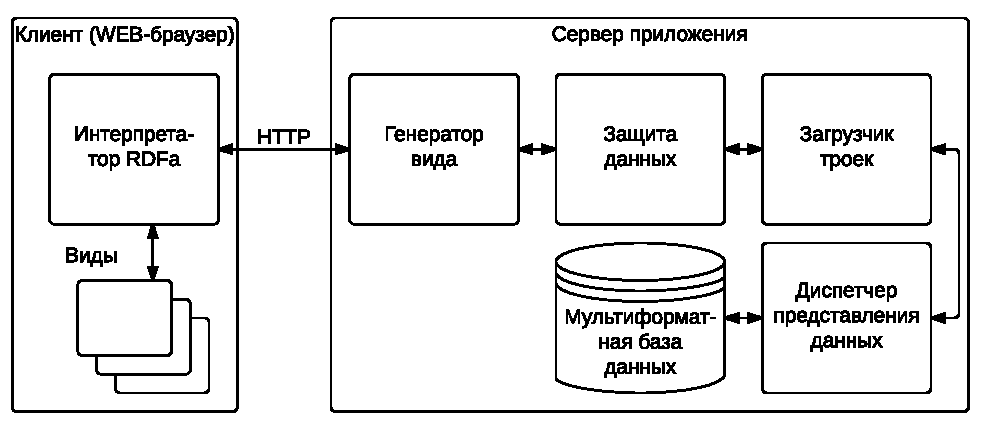
\includegraphics[width=0.8\linewidth]{peixe-architecture-ru-1.pdf}
% where an .eps filename suffix will be assumed under latex,
% and a .pdf suffix will be assumed for pdflatex; or what has been declared
% via \DeclareGraphicsExtensions.
\caption{Архитектура ядра программной системы}
\label{architecture}
\end{figure}

\subsection{Используемые инструментальные средства}
\label{sec:instr}

\e[cyan]{Здесь продолжаем писать то, на чем будем писать и как что
  будем делать. Т.е. некоторые технические детали.}

Ориентация проекта на решение прикладных задач приводит к следующему
набору требований к целевым свойствам программного продукта.
\begin{enumerate}
\item Свободное (open-source) приложение \e{Цель --- привлечь
    программистскую общественность к проблеме разработки и
    реинжениринга полисистемы онтологий, порождаемой продвинутыми пользователями}.
\item Программа должна иметь две реализации\,: локальную и в виде интернет-приложения.
\item Северная часть интернет-приложения \e{должна устанавливаться и
    функционировать} в \e{недорогом хостинге}.  \label{e12:p2}
\item В следствие п.~\ref{e12:p2} необходима поддержка различных
  \e{провайдеров} баз данных для хранения троек.
\end{enumerate}

Современные ресурсы, предоставляемые коммерческими
интернет-провайдерами, \e{ранжируются} от предоставление ресурсов для
процесса веб-сервера до виртуального и облачного хостинга.  Недорогим
классом является первый вариант, называемый виртуальным хостингом.
При этом в качестве популярной платформы для разработки программного
выступает комбинация языка программирования PHP, сервера баз данных
MySQL, функционирующих под управлением операционной системы Linux.
Кроме того, современные интернет-приложения \e{со стороны серверной
  части} используется JavaScript.

\e{Кристина - переведи на русский свой текст.}

[The flexibility and minimum resources and administration requirements criteria are of very importance to choosing database providing information resources storage as triples.  The database management systems as DB2, Oracle and SQL Server cannot fulfill requirements because after running the operation is performed as a separate process.  Also application and DBMS interaction should be implemented through interprocess communication form.

Solution to these problems is achieved by using the built-in database management systems that provide communication with the application at the same level of address space.  This allows the application based on the built-in database to be efficient and autonomous.

Kyoto Cabinet is a library of routines for managing a database.  The database is a simple data file containing records, each is a pair of a key and a value.  Every key and value is serial bytes with variable length.  Both binary data and character string can be used as a key and a value.  Each key must be unique within a database.  There is neither concept of data tables nor data types.  Records are organized in hash table or B+ tree.  \cite{b1}

Availability of funds to work with triplets described in the standard RDF is an advantage database management system Kyoto Cabinet over other embedded systems is.  In this case the developer does not need to spend time on design and implementation of the data model so that its performance on this task is increased.

1.	Kyoto Cabinet. URL: http://fallabs.com/kyotocabinet/ (дата обращения: 20.02.2014).]

\e{Далее (Кристина) надо рассмотреть программное обеспечение, необходимое для
  реализации проекта на PHP + (MySQL | PostgreSQL | KyotoCabinet) +
  ZPT (PHP, \url{http://phptal.org/manual/ru/}) и найти для PHP библиотеку как rdflib. Еще надо описать
  библиотеки rdf и т.п. на клиентской (JavaScript) части (\url{http://en.wikipedia.org/wiki/Template_Attribute_Language}). }

\begin{figure}[!t]
\centering
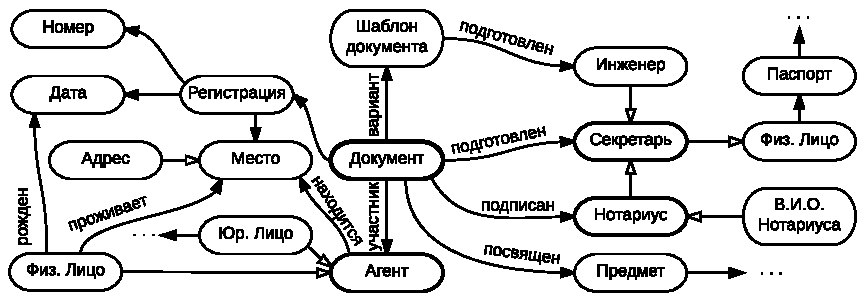
\includegraphics[width=0.8\linewidth]{DocumentOntology-ru.pdf}
% where an .eps filename suffix will be assumed under latex,
% and a .pdf suffix will be assumed for pdflatex; or what has been declared
% via \DeclareGraphicsExtensions.
\caption{Верхний уровень онтологии предметной области представления
  нотариального документа}
\label{notaryontology}
\end{figure}

\section{Подобные проекты и дальнейшее развитие результатов}

Среди известных проектов в той или иной степени использующей средства
интерактивного построении семантической разметки текстовых документов
выделяется “Semantic MediaWiki”.  Здесь редактор текстового
представления страниц вики расширен возможностью задания частям текста
семантических аннотаций.  Для этого разработан специальный формат
разметки.  Аннотации используются механизмом поиска информации по
страницам вики на сайте \cite{b1:13}.

В сравнении с предыдущей разработкой в проекте OntoWiki \cite{b:2:14}
получены аналогичные результаты, но с другой \e{отправной точки}.
OntoWiki основывается на идее использования логического слоя
(семантической сети) для представления всей информации на сайте
\e{(как у нас)}.  Логический слой редактируется при помощи форм ввода,
порождаемых автоматически на основе существующих в системе словарей
(term sets).  Пользователю разрешено редактирование только один
текстовый атрибут \texttt{lod:content}, где разрешено использование
формата HTML.  Такой HTML-текст не имеет никакого отношения к
существующей логической структуре текста, представляемого, в конечном
счете, в виде документа web.   Текст редактируется при помощи
визуального (WYSIWYG) редактора, встроенного в OntoWiki.  Проект
осуществляет технологическую поддержку развития социальной сети,
\e{базирующейся на формате Linked Data}.

Представленный в данной статье материал представляет собой развитие
идей OntoWiki в направлении \e{
engine to support a natural representation of the document content,
visual editing of the content, conserving the logical layer;
implementation of the data and knowledge acquisition on the base of
modification analysis.}  Шаблоны представления чайте документов в
OntoWiki хранятся в специальных структурах данных вне онтологии и не
зависят от контекста документа.  Преимущество нашего подхода состоит в
том, что представление, будучи полноценным элементом онтологии, могут
быть логически выведены из иерархии наследования.  Кроме того,
использование \e{Most of the
interrelations between text content and its logical structure are
expressed in RDFa}.

\e{Ведение диалога}
\url{http://www.sri.com/sites/default/files/uploads/publications/pdf/687.pdf}
\url{http://www.jfsowa.com/pubs/semnet.htm}


Дальнейшее развитие проекта направлено на реализацию функций
интеллектуального анализа данных схожих документов для выявления
зависимостей между значениями атрибутов (объектов), встречающихся в
тексте.  Результаты этого анализа можно использовать для принятия
решения о варианте формата представления троек.  Если в некотором
множестве атрибутов замечены зависимости, то этот набор атрибутов
вероятно возможно хранить в виде таблицы реляционной базы данных.  Для
этого необходимо выделить детерминант согласно методу функциональных
зависимостей.  В отличие от \e{обычного использования} этого метода,
когда функциональные зависимости выявляются на основе \e{[?как она
  называется?]} интерпретации свойств атрибутов, в данном случае эти
зависимости выявляться при помощи методов многомерного статистического
анализа данных в виде корреляций.

The abstract layer of information modeling of the knowledge
acquisition is a category of system complexes (configurations) [15],
which is perfectly embody common metamodel of the ontologies as well
as supply additional structural and functional properties. Developing
the theory further one can connect the ontology devised during the
document preparation process to the stage of UML-modelling of
information system, which automates the processes of the domain.

\e{Представление результатов разметки в виде UML-диаграмм и переход к
  CASE- и MDE-средствам. }

\conclusion

\e{Общие слова о разрабатываемой технологии и задачи, решаемой ...}

Рассмотрен подход к представлению логического слоя тестового
содержимого документа (или электронного ресурса), базирующийся
использовании полисистемы онтологий \e[cyan]{что это дает?}, представленных в формате RDF
(Resource Description Framework).  Формат позволяет как хранить
отношения между сущностями, описывающими семантику содержимого
документа, так и шаблоны для преобразования логических структур в
текстовые фрагменты документа.  Изложена программная методика этого преобразования
(\e{отрисовки, rendering}).  В результате преобразования
сгенерированный текст также содержит данные семантической разметки в
формате RDFa.  Эти данные предполагается использовать на стороне
клиента (веб-браузера) для организации интерфейса пользователя, в
частности для редактирования данных логического слоя.

В основной части работы рассмотрена методика организации интерактивного
процесса формирования логического слоя содержимого на основе
интеллектуального анализа изменений различных версий документа,
порожденных пользователем.  Рассмотрена задача ведения диалога с
пользователем, целью которого является дополнение существующей
семантической модели (логического слоя представления содержимого)
новыми объектами и отношениями.  Диалог с пользователем ведется при
помощи логического вывода на сетевом представлении полисистемы онтологий.

\e[cyan]{Представление программной части: архитектура и требования,
  которым хочется соответствовать.}

В качестве практического тестового приложения предложена реализация
автоматизации деятельности секретарей нотариальной конторы.
Представление документов, подготавливаемых в конторе, отличается
сбалансированностью формализуемой и неформализуемой частями текста.
Кроме того, на базе разрабатываемой технологии возможно построение
социальной сети обмена текстами документов.

\e{Чего, собственно, хочется добиться?} Разработка методики извлечения
знаний из документов.

% use section* for acknowledgement
\thanks Результаты исследований получены при поддержке Интеграционного
междисциплинарного проекта СО РАН №17 «Создание сервисов и
инфраструктуры научных пространственных данных для поддержки
комплексных междисциплинарных научных исследований Байкальской
природной территории».

\begin{thebibliography}{11}
\bibitem{TBL2001} T. Berners-Lee, J. Hendler and O. Lissila. \emph{The Semantic Web A new form of Web content that is meaningful to computers will unleash a revolution of new possibilities.}\hskip 1em plus 0.5em minus 0.4em\relax  Scientific American, May 17, 2001, pp.1-18. URL: http://sciam.com/article.cfm?articleID=00048144-10D2-1C70-84A9809EC588EF21. (access date: 05.09.2013).
\bibitem{q1}
Social network - Wikipedia, the free encyclopedia. URL: \url{http://en.wikipedia.org/wiki/Social_network} (access date: 20.08.2013).
\bibitem{q2}
Chameleon – Chameleon 2.10 documentation. \url{http://chameleon.readthedocs.org/en/latest/} (access date:  20.08.2013).
\bibitem{q3}
Virtuoso Open-Source Edition URL: \url{http://virtuoso.openlinksw.com/dataspace/doc/dav/wiki/Main/} (access date: 30.05.2013).
\bibitem{q4}
PIZZA Protege OWL tutorial at Manchester (School of Computer Science - The University of Manchester)  URL:\url{http://owl.cs.manchester.ac.uk/tutorials/protegeowltutorial/} (access date: 20.09.2013).
\bibitem{q5}
SWI-Prolog's home. URL: \url{http://www.swi-prolog.org/} (access date: 20.08.2013).
\bibitem{q6}
The Protégé Ontology Editor and Knowledge Acquisition System. URL: \url{http://protege.stanford.edu/} (access date: 20.08.2013).
Semantic MediaWiki. URL: \url{http://semantic-mediawiki.org/} (access date: 20.08.2013).
\bibitem{q7}
N.Heino, S.Tramp, N.Heino, S.Auer. Managing Web Content using Linked Data Principles – Combining semantic structure with dynamic content syndication. Computer Software and Applications Conference (COMPSAC), 2011 IEEE 35th Annual. pp. 245 - 250. URL:\url{http://svn.aksw.org/papers/2011/COMPSAC_lod2.eu/public.pdf} (access date: 30.05.2013).
\bibitem{q8}
Cherkashin E.A., Paramonov V.V., et al, Model Driven Architecture is a Complex System, E-Society Journal Research and Applications. Volume 2, Number 2, 2011, pp. 15-23.
\bibitem{q9}
Father
\bibitem{granin} Гранин с его представлением иконок.

% Format examples.
\bibitem{m1} Автор И.О. Название книги --- М.: Издательство, 2002. --- 700~с.
\bibitem{m2} Автор И.О. Статья // В книге --- Ижевск: Издательство, 2011. --- С.~71-90.
\bibitem{m3} Сайт ТИПД-2014 // \url{http://itpa2014.conf.udsu.ru/}
\bibitem{b2:2} Microformats. URL:http://microformats.org/ (дата обращения\,: 30.05.2013).
\bibitem{b2:5} Model–view–controller --- Wikipedia, the free encyclopedia. URL: http://en.wikipedia.org/wiki/Model-view-controller (дата обращения\,:20.09.2013).
\bibitem{b2:6} Sandhu "Role-based access control." Advances in computers. 46 (1998): 237-286.

\bibitem{b2:7} T.Berners-Lee, R. Cyganiak, et.al. On Integration Issues of Site-Specific APIs into the Web of Data. DERI Technical Report 2009-08-14. URL: http://linkeddata.deri.ie/sites/linkeddata.deri.ie/files/rw-wod-tr.pdf (access date: 20.09.2013).
\bibitem{b2:8} Virtuoso Open-Source Edition URL: http://virtuoso.openlinksw.com/dataspace/doc/dav/wiki/Main/ (access date: 30.05.2013).
\bibitem{b2:13} Semantic MediaWiki. URL: http://semantic-mediawiki.org/ (access date: 20.08.2013).
\bibitem{b2:14} N.Heino, S.Tramp, N.Heino, S.Auer. Managing Web
  Content using Linked Data Principles – Combining semantic structure
  with dynamic content syndication. Computer Software and Applications
  Conference (COMPSAC), 2011 IEEE 35th Annual. pp. 245 -
  250. URL:http://svn.aksw.org/papers/2011/COMPSAC\_lod2.eu/public.pdf
  (access date: 30.05.2013).
\bibitem{b2:15} Cherkashin E.A., Paramonov V.V., et al, Model Driven Architecture is a Complex System, E-Society Journal Research and Applications. Volume 2, Number 2, 2011, pp. 15-23.
\end{thebibliography}

% that's all folks
\end{document}

%% Local Variables:
%% eval: (ispell-change-dictionary "ru_RU_hunspell")
%% TeX-master: t
%% TeX-PDF-mode: 1
%% TeX-source-correlate-mode: 1
%% TeX-source-correlate-start-server: nil
%% End:
